

\begin{figure*}[ht!]
	\centering
	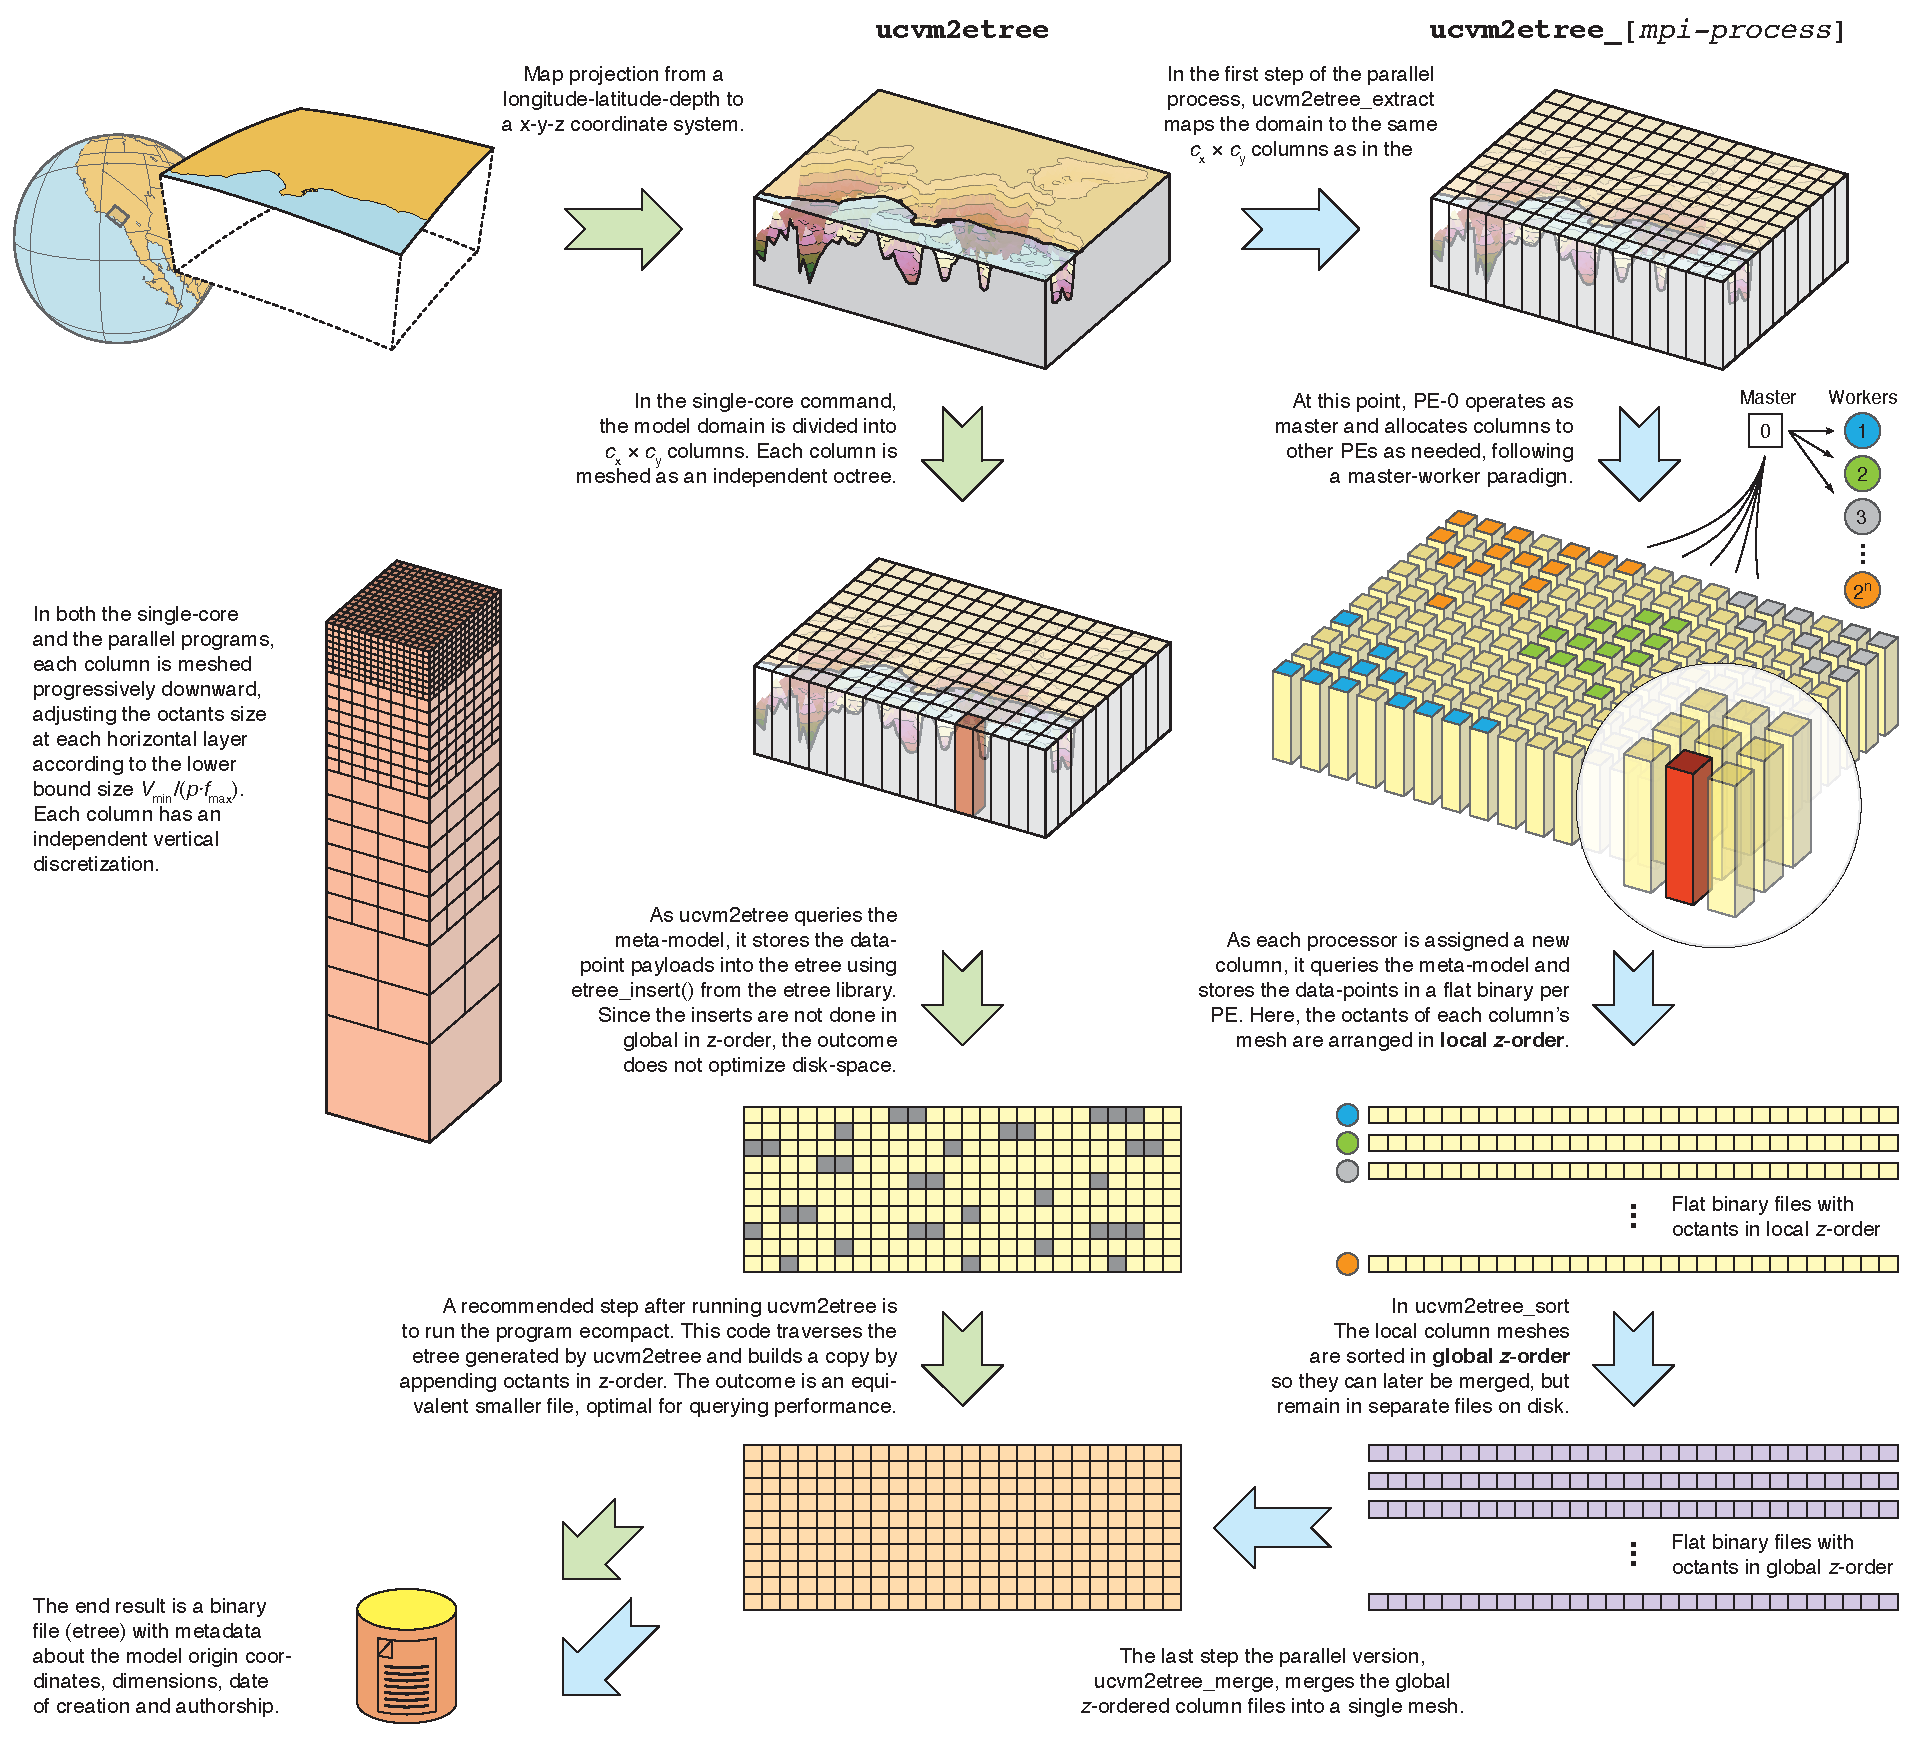
\includegraphics
		[width=\textwidth]
		{figures/pdf/ucvm-to-etree}
	\caption{Construction of an pseudo-unstructured mesh in the Etree database format using the program \texttt{ucvm2etree} and its MPI equivalent processes \texttt{ucvm2etree\_extract}, \texttt{ucvm2etree\_sort} and \texttt{ucvm2etree\_merge}. An important aspect of the meshing-to-etree process is that the discretized information payload (\vs{}, \vp{}, and $\rho$) is stored at the octants in the octree structure. The querying and assignment process mapps the information queried at the center of each octant to the whole volume enclosed by the octant.}
	\label{fig:etrees}
\end{figure*}
% ---------------------------------------------------------------------------------------------


\subsection{Creating Etree Databases}

The framework may also be utilized to generate a semi-unstructured octree in the \textit{etree} database format \citep{Tu_2003_Tech} using the command-line program \texttt{ucvm2etree}. Two etree database formats are supported: the Hercules format, and the SCEC format. These two formats differ in the format of their metadata signatures, and more important, in the map projection used to discretize the domain. The Hercules format utilizes a projection that corresponds to a bilinear interpolation based on the four corner coordinates that define the surface bounding box in geographical coordinates. The SCEC format, on the other hand, supports any map projection available in the Proj.4 projection library.

The construction of an etree proceeds as shown in Figure \ref{fig:etrees}, which follows some of the basic ideas first proposed in the implementation by \citet{Taborda_2007_Proc}. The user specifies the extents of the etree by describing the $x$-$y$-$z$ dimensions of the domain in meters, as well as providing the geographical data necessary to define a bounding box on the Earth's surface. In the case of the Hercules format this consists of the coordinates of the bounding box on the Earth's surface. In the case of the SCEC format, this is done similarly as in the case of the structured meshes explained before. Using the correspoinding bilinear or Proj.4 projection, this surface bounding box is mapped to the $x$-$y$ plane of the domain. The $z$ dimension of the domain is interpreted as depth from the free surface. In this way, any ($x,y,z$) coordinate in the domain may be transformed to a (\textit{latitude},\textit{longitude},\textit{depth}) coordinate relative to the Earth's surface. It is assumed that the user has pre-computed the domain dimensions such that they reflect the actual distances in the geographic bounding box (using any preferred projection or spheroid model). Note, however, that the octree format places restrictions on the possible valid domain sizes \citep{Tu_2003_Tech, Taborda_2007_Proc}.

% *****

% I changed the above paragraph somewhat considerably, so I am keeping a copy of the old version here at least during one git submission

%For the purposes of this discussion, we shall describe the generation of a Hercules-format Etree database based on \citet{Taborda_2007_Proc}. Construction of such an Etree proceeds as shown in Figure \ref{fig:etrees}. The user specifies the extents of the Etree by describing the x-y-z dimensions of the domain in meters, as well as providing the geographical coordinates of a bounding box on the Earth's surface. This surface bounding box is mapped to the x-y plane of the domain using bilinear interpolation. The z dimension of the domain is interpreted as depth from the free surface. In this way, any $(x,y,z)$ coordinate in the domain may be transformed to a $(latitude, longitude, depth)$ coordinate relative to the Earth's surface. It is assumed that the user has pre-computed the domain dimensions such that they reflect the actual distances in the geographic bounding box (using any preferred projection or spheroid model). Note, however, that the octree format places restrictions on the possible valid domain sizes \citep{Tu_2003_Tech, Taborda_2007_Proc}.

% *****

This domain is then spatially decomposed at a coarse-grained level, dividing the volume into a two-dimensional logical grid of rectangular cuboids (columns) aligned with the $x$-$y$ plane of the original domain, with each column having a fixed size. This decomposition assists in parallelization since the material properties for a particular column can be extracted independently from the others. The number of columns in this logical grid is selectable by the user, subject to two constraints to preserve the octree format. First, the length and width of the columns must be equal. Second, the number of columns along the $x$ and $y$ axis must be a power of two.

With this coarse decomposition complete, each column of the original domain may then be processed in sequence by \texttt{ucvm2etree}, or in parallel, as is the case with the MPI version of this utility (see Figure \ref{fig:etrees}). To extract the material properties for a column, the program further decomposes the column into a collection of octants, maps the center ($x$,$y$,$z$) coordinate of each octant to its corresponding geographic coordinates, and then queries the user-provided list of velocity models to determine the (\vp{},\vs{},$\rho$) payload for each octant. The octants are processed in a top-down fashion, starting at the surface and ending at the maximum depth of the domain. Filled octants are inserted into the etree database via the etree API. Note that as opposed to the structured grids explained above, where the query-point and the grid-point have a 1-to-1 mapping relationship, here it is the volume contained by an octant the one who takes the query-point payload properties.

This fine-grain decomposition into octants is an adaptive process that depends on the shear-wave velocities (\vs{}) encountered within that column as well as four parameters provided by the user: \vsmin{}, a floor \vs{} for purposes of bounding octant sizes to a minimum size; \fmax{}, the maximum simulation frequency to support; $p$, the desired number of points per wavelength to be used in a simulation model; and $s_{_{\max}}$, the maximum octant size to allow. Based on these parameters, the program determines the range of octant sizes to allow within a column. The upper bound is determined by:
%
\begin{equation}
\label{eq:octant_upper}
	s_{_{\mathrm{upper}}} = \min ( l_c, s_{_{\max}} )
	\hspace{0.3em},
\end{equation}
%
where $l_c$ is the column length. The lower bound is given by:
%
\begin{equation}
\label{eq:octant_lower}
	s_{_{\mathrm{lower}}} = \frac{ V_{\mathrm{S}_{\min}} }{ p f_{_{\max}}}
	\hspace{0.3em}.
\end{equation}
%
As the octree format places constraints on valid octant sizes, these two bounds are normalized with the relation:
%
\begin{equation}
\label{eq:octant_size}
	s_{_{\mathrm{octant}}} = \frac{ l_d }{ 2^{ \left( \left\lceil \log_{2} \left( \frac{l_d}{s} \right) \right\rceil \right)} }
	\hspace{0.3em}.
\end{equation}
%
Here, the variable $l_d$ is the domain length (longest side); and the variable $s$ is the size to normalize, which is either $s_{_{\mathrm{upper}}}$ or $s_{_{\mathrm{lower}}}$, corresponding to the upper and lower bounds, respectively.

With these bounds established, the program successively queries two-dimensional slices of octants, starting at the column surface and stepping downward to greater depths. Initially, the octants are of size $s_{_{\mathrm{lower}}}$ (maximum resolution). Then, as the program progresses downwards, the octants are resized based on the actual \vs{} values encountered within a slice. After each slice is queried, the minimum \vs{} found within is inserted into equation (\ref{eq:octant_lower}) and then normalized with (\ref{eq:octant_size}) to yield an updated octant size. If this new size differs from the current size while still falling within the $s_{_{\mathrm{lower}}}$ and $s_{_{\mathrm{upper}}}$ bounds, and if this size fits in the remaining vacant space of the octree, then the slice is re-queried at the new size. Otherwise, the slice of octants is accepted as queried and inserted into the etree database.

This adaptive refinement continues as the program steps down through the column. As \vs{} values typically increase with depth, the program will tend to select larger octant-sizes as it proceeds deeper into the column (as illustrated int eh column shown in Figure \ref{fig:etrees}, to the left). This refinement algorithm ensures that each column is extracted at a resolution which supports the maximum simulation frequency, while at the same time allowing for considerable space savings at depth. Since the column properties are defined by the user, but the meshing of each column is adaptive, we defined the output of this process as a semi-unstructured mesh.

The MPI implementation of \texttt{ucvm2etree} consists of a workflow with three programs: \texttt{ucvm2etree\_extract}, \texttt{ucvm2etree\_sort}, and \texttt{ucvm2etree\_merge}. The program \texttt{ucvm2etree\_extract} performs the same spatial decomposition and velocity model querying as described above, with the change that each column is extracted independently by each processor and the octants are temporarily saved to disk in flat binary files. The program \texttt{ucvm2etree\_sort} locally sorts the octants of each column by their location code. The last program in the workflow, \texttt{ucvm2etree\_merge}, performs a merge sort of the locally sorted columns, such that rank 0 inserts the ordered octants one at a time into the etree database \citep[in its natural $z$-order; see][]{Tu_2003_Tech}. Since the octants are globally sorted at this point, the insertion is simply an append operation. 

This scheme, while more complicated than the sequential program, allows extraction to occur in parallel while \texttt{ucvm2etree\_merge} utilizes the most efficent insertion method provided by the etree library (\texttt{etree\_append}), which operates in $z$-order. By contrast, when running the sequential program, storage of the payload into the etree is handled with the library function \texttt{etree\_insert}, in the order queries to the meta-model are done. This is not the same order as that of the etree. As a result, the binary file contains ``unused'' disk space. The resulting etree can be optimized by running the program \texttt{ecompact}, which traverses an etree and creates a copy in the correct compact order (see Figure \ref{fig:etrees}). Further size optimization can be achieved on any etree by running the program \texttt{ecoalesce}, which combines octants with identical properties into larger units, thus breaking the initial sub-structure and optimizing disk-space to create truly unstructured models. Both \texttt{ecompact} and \texttt{ecoalesce} were developed as part of an effort independent of the UCVM platform development \citep{Schlosser_2008_Proc}, which inspired some of the ideas used in the UCVM etree features.
